\section{User Bias for Early Content}

\begin{figure*}[!tb]
\centering
\begin{subfigure}{.3\textwidth}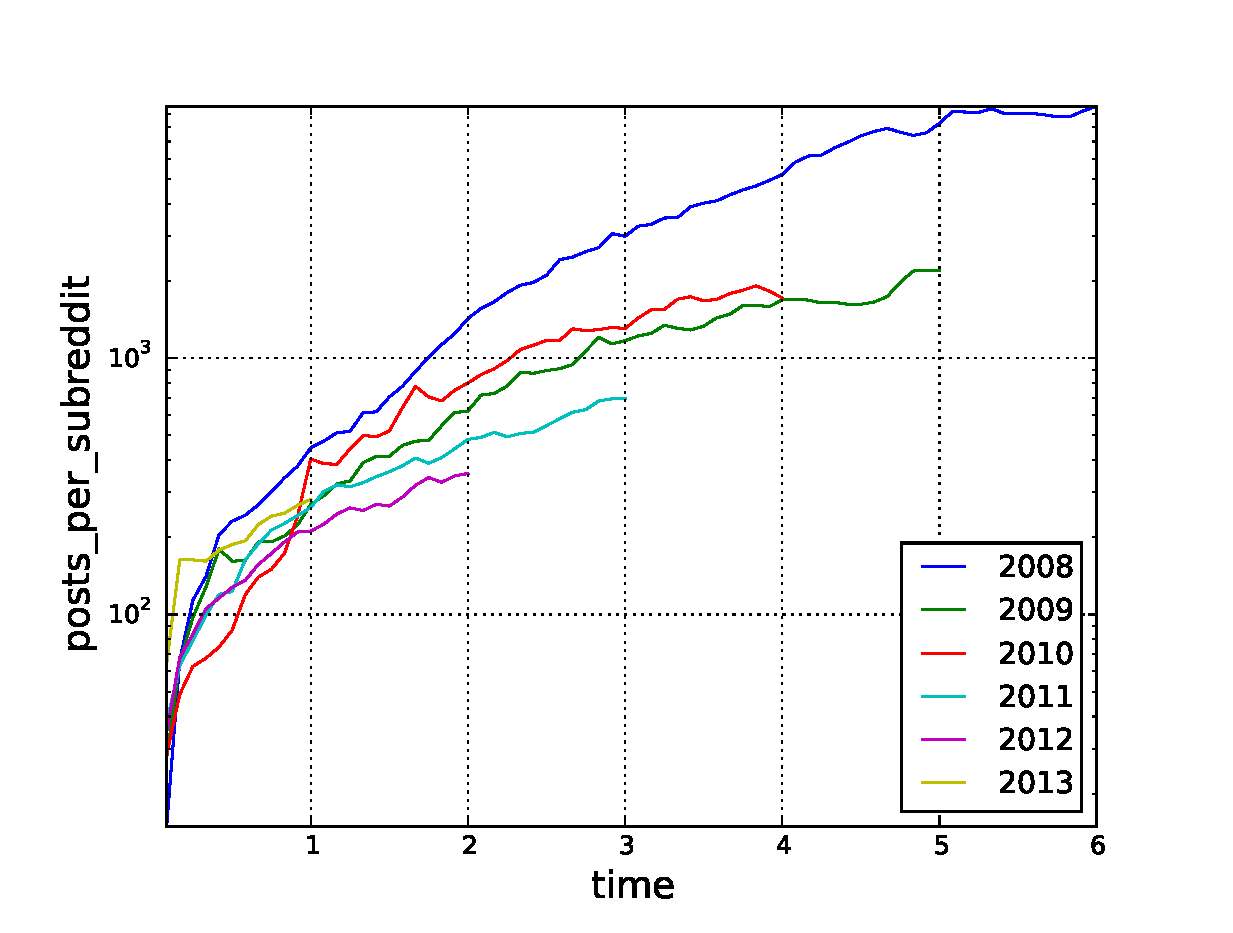
\includegraphics[scale=0.285]{./images/posts_per_subreddit_cohorts.eps}\caption{}\end{subfigure}
\begin{subfigure}{.3\textwidth}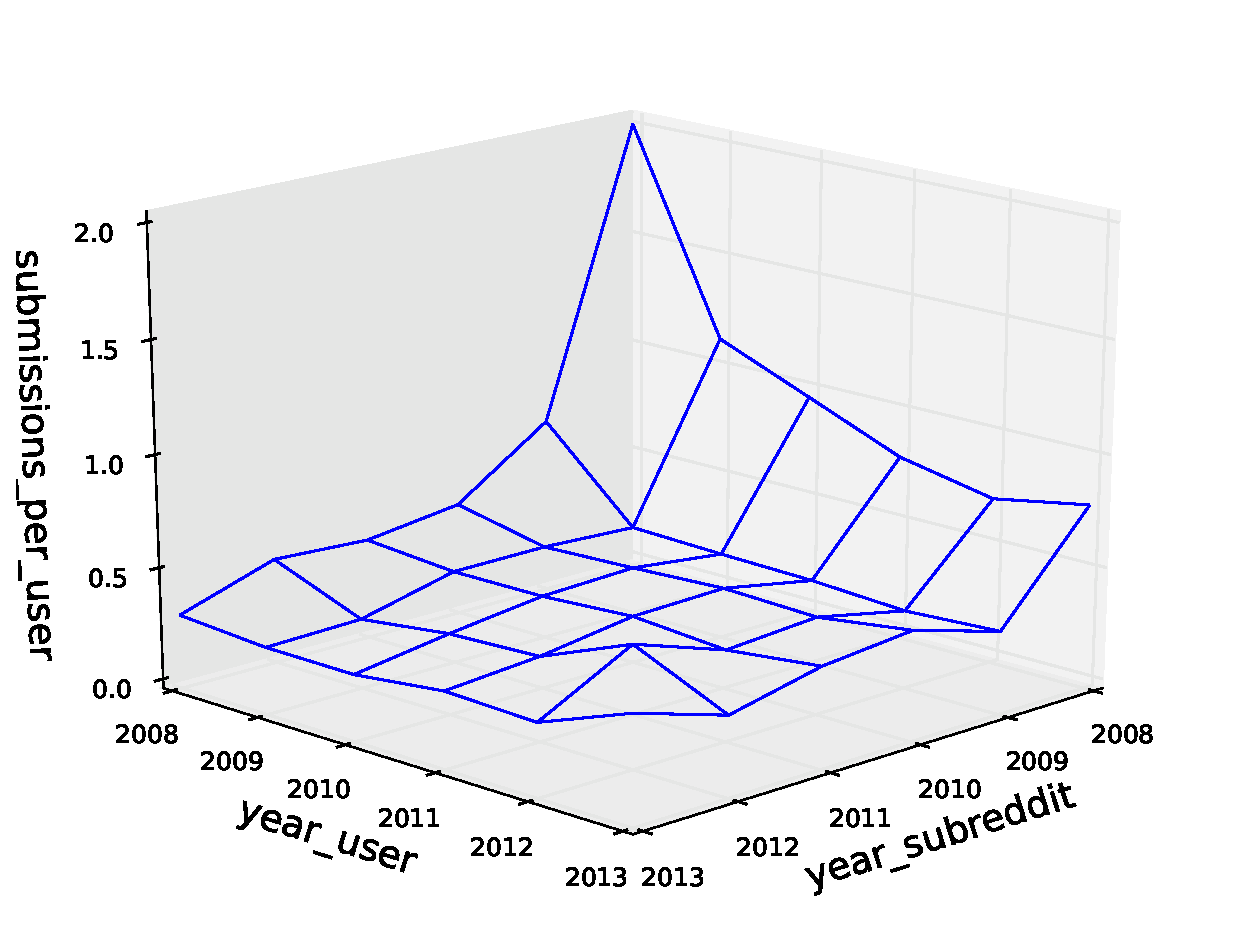
\includegraphics[scale=0.285]{./images/user_subreddit_submissions_cohorts.eps}\caption{}\end{subfigure}
\begin{subfigure}{.3\textwidth}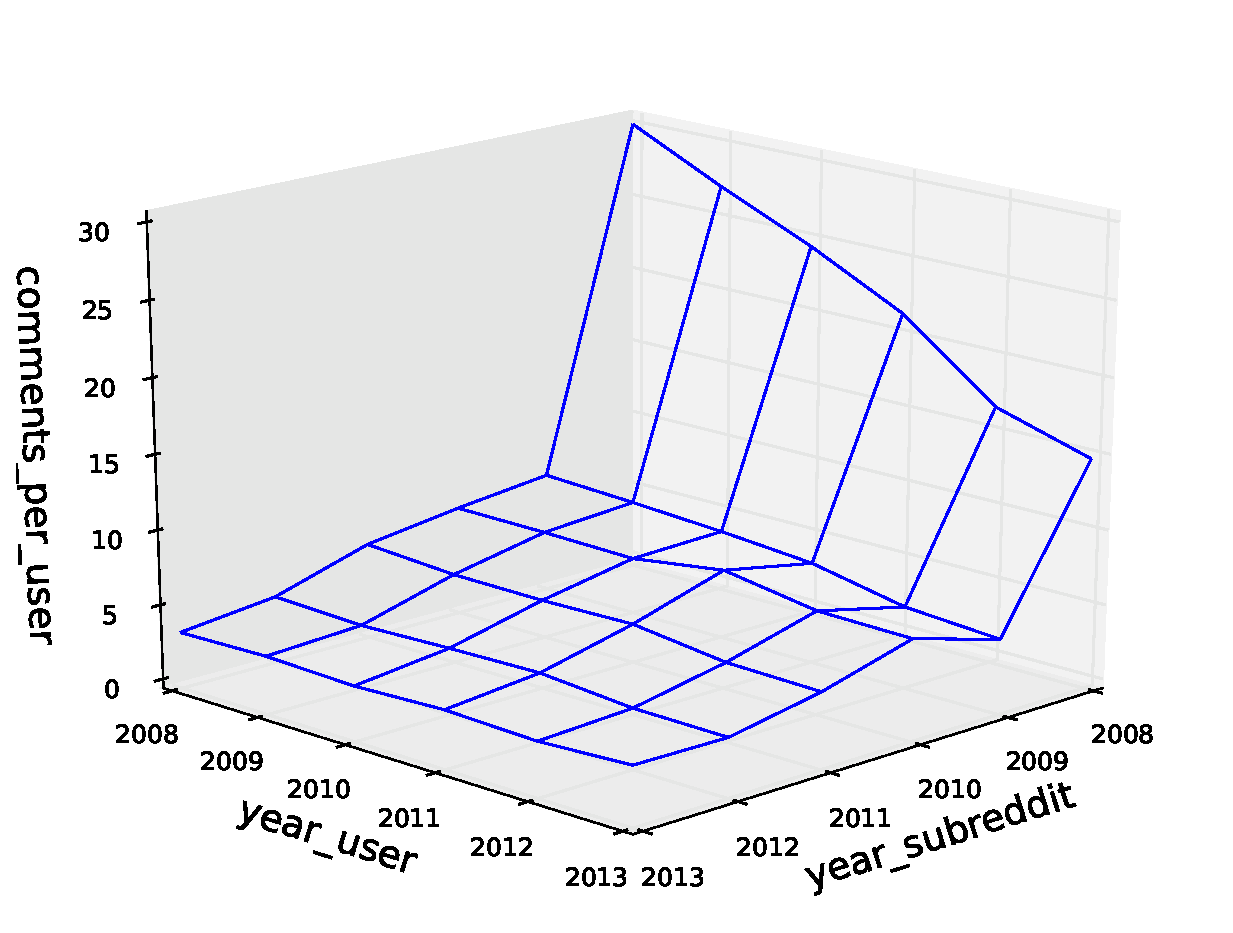
\includegraphics[scale=0.285]{./images/user_subreddit_comments_cohorts.eps}\caption{}\end{subfigure}
\caption{Caption}
\label{fig:user_subreddit_submissions_cohorts}
\end{figure*}

The cohort a user belongs to has a significant impact to the user posting behavior, but that does not give us a picture of how these users coexist in the current community. An interesting hypothesis that we could imagine is that users from a particular cohort are more interest in the communities from a particular cohort. We now look at the interplay between user and subreddit cohorts. 

An initial hypothesis would be that users would be interested in the communities that were being created at the same time they joined the network. To test for that, Figures N and N show the number of submissions and comments per user, respectively, based on the user and subreddit cohorts.

It is possible to see that users' behavior, independently of the cohort, are biased to subreddits created on 2008. 2008 users' submissions are particularly more biased to 2008 subreddits. This might be due to the fact that these surviving users play a much more central role in these communities (moderators or key contributors) since they are more likely to be there from the start.

These observations allow us to conclude that, in the case of reddit, there are key subreddits that were created in 2008 that are the main focus of attention of all the users, although this is decreasing as new users join the network. Our hypothesis would not hold true in this case. This, however, might not hold true for other social networks, in which the communities or the content at the time at which users join the network might be their main focus of attention, highlighting again the importance of performing a cohort based analysis.
